\section{Muhammad Reza Syachrani - 1174084}
\subsection{Teori}
\begin{enumerate}

	\item Jelaskan dengan ilustrasi gambar sendiri apa itu generator dengan perumpamaan anda sebagai mahasiswa sebagai generatornya.
	\hfill\\
Tugas Generator sekarang sedang dibuat untuk membuat koleksi gambar palsu, yang saat ini dilihat oleh Diskriminator. Diskriminator tidak dapat membedakan antara yang asli dan yang palsu. Untuk ilustrasi, lihat gambar berikut:

\begin{figure}[H]
    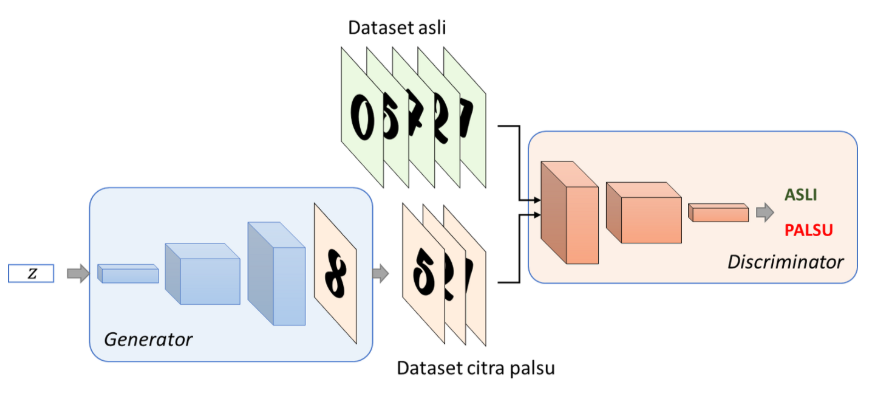
\includegraphics[width=12cm]{figures/1174084/8/teori1.png}
    \centering
    \caption{Teori 1}
\end{figure}

\item Jelaskan dengan ilustrasi gambar sendiri apa itu diskriminator dengan perumpamaan dosen anda sebagai diskriminatornya
	\hfill\\
	Diskriminator adalah CNN yang menerima input gambar yang dimiliki dan menghasilkan angka biner yang meminta input gambar, lalu menghasilkan gambar dari dataset asli atau menghasilkan gambar palsu. Untuk ilustrasi, lihat gambar berikut:  

\begin{figure}[H]
    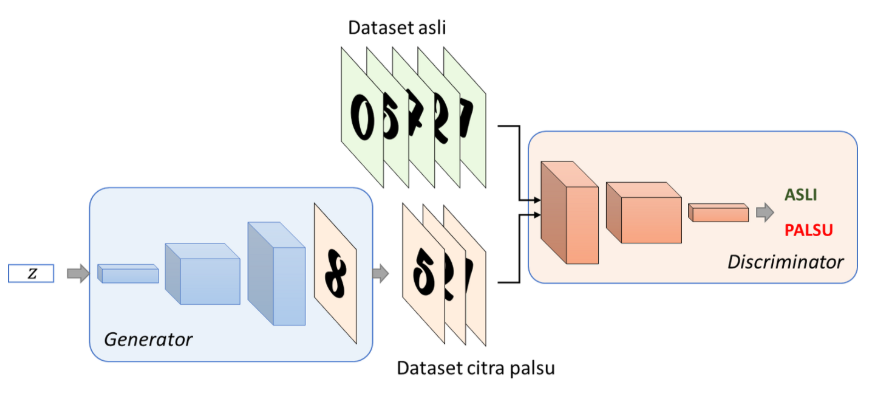
\includegraphics[width=12cm]{figures/1174084/8/teori1.png}
    \centering
    \caption{Teori 2}
\end{figure}

\item Jelaskan dengan ilustrasi gambar sendiri bagaimana arsitektur generator dibuat
	\hfill\\
	Aksitektur generator dibuat bisa dijelaskan pada gambar berikut : 

\begin{figure}[H]
    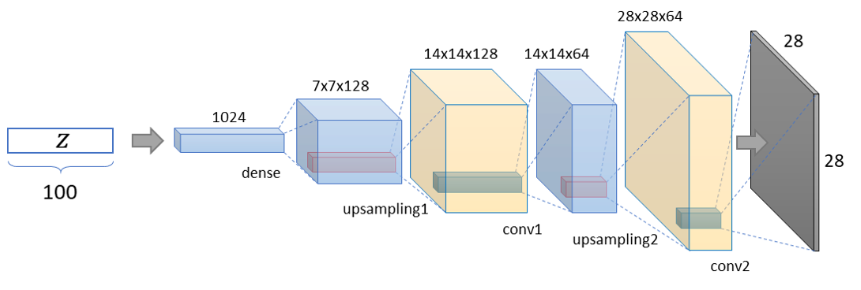
\includegraphics[width=12cm]{figures/1174084/8/teori3.png}
    \centering
    \caption{Teori 3}
\end{figure}

\item Jelaskan dengan ilustrasi gambar sendiri bagaimana arsitektur diskriminator dibuat.
\hfill\\
	Aksitektur diskriminator dibuat bisa dijelaskan pada gambar berikut : 
	
\begin{figure}[H]
    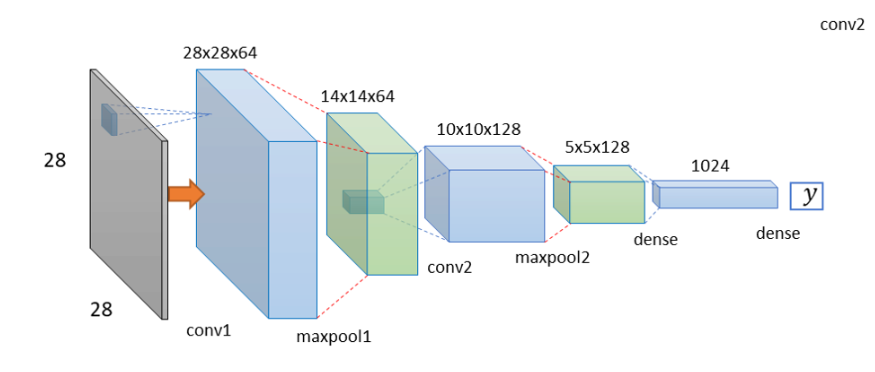
\includegraphics[width=8cm]{figures/1174084/8/teori4.png}
    \centering
    \caption{Teori 4}
\end{figure}

\item Jelaskan dengan ilustrasi gambar apa itu latent space.
	\hfill\\
	Latent space dijelaskan pada gambar berikut :

\begin{figure}[H]
    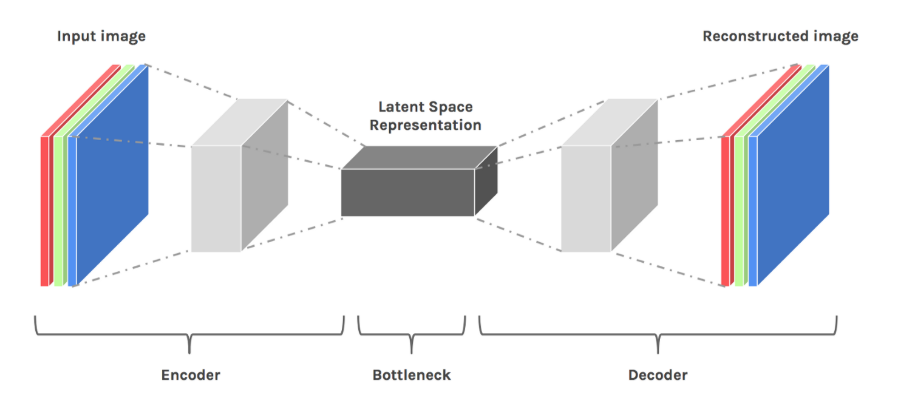
\includegraphics[width=8cm]{figures/1174084/8/teori5.png}
    \centering
    \caption{Teori 5}
\end{figure}

\item Jelaskan dengan ilustrasi gambar apa itu adversarial play
	\hfill\\
	adversial play ialah persaingan antara generator dan diskriminator. bisa dilihat pada ilustrasi gambar berikut:
	
\begin{figure}[H]
    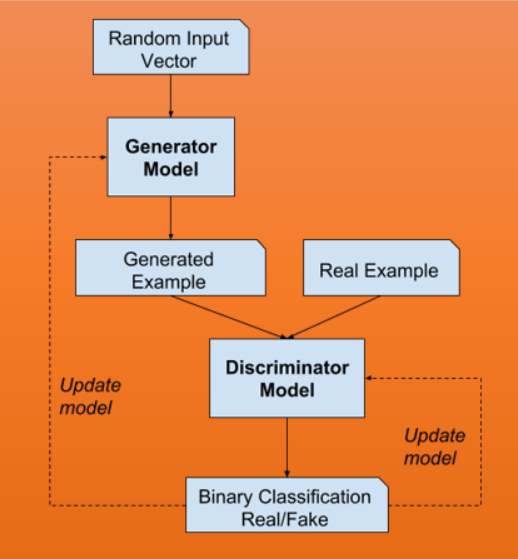
\includegraphics[width=8cm]{figures/1174084/8/teori6.png}
    \centering
    \caption{Teori 6}
\end{figure}

\item Jelaskan dengan ilustrasi gambar apa itu Nash equilibrium.
	\hfill\\
	Nash equilibrium konsep teori permainan di mana hasil optimal dari permainan adalah di mana tidak ada pemain yang memiliki insentif untuk menyimpang dari strategi yang dipilih setelah mempertimbangkan pilihan lawan
	Nash equilibrium pada gambar berikut :
		
\begin{figure}[H]
    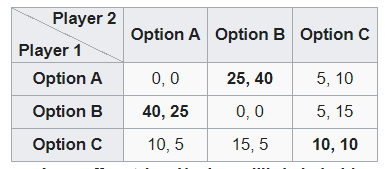
\includegraphics[width=8cm]{figures/1174084/8/teori7.png}
    \centering
    \caption{Teori 7}
\end{figure}

\item Sebutkan dan jelaskan contoh-contoh implementasi dari GAN
	\hfill\\
	Implementasi 3DGAN yaitu pada MAPS dan juga IKEA. Karena pada maps dan juga ikea sudah menerapkan bentuk 3 dimensi yang bisa lebih menarik perhatikan pengguna.
	
\item Berikan contoh dengan penjelasan kode program beserta gambar arsitektur untuk membuat generator(neural network) dengan sebuah input layer, tiga hidden layer(dense layer), dan satu output layer(reshape layer).
	\hfill\\
	
	
\begin{figure}[H]
    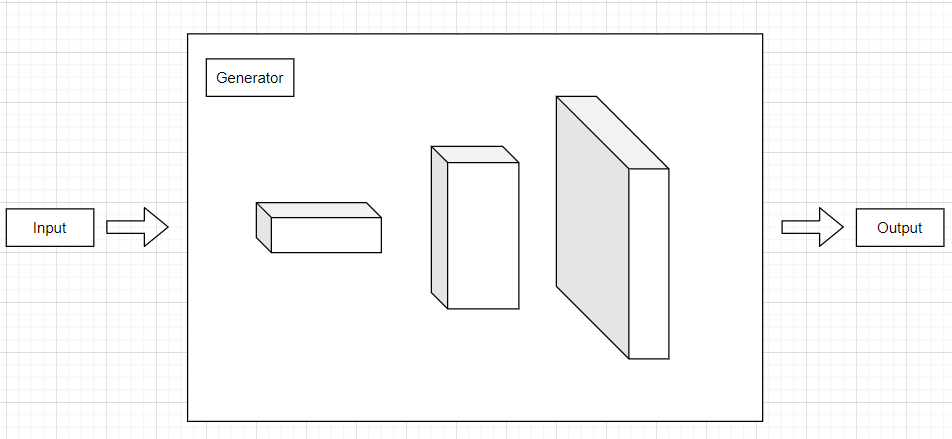
\includegraphics[width=8cm]{figures/1174084/8/teori9.png}
    \centering
    \caption{Teori 9}
\end{figure}


\item Berikan contoh dengan ilustrasi dari arsitektur dikriminator dengan sebuath input layer, 3 buah hidden layer, dan satu output layer.
	\hfill\\

\begin{figure}[H]
    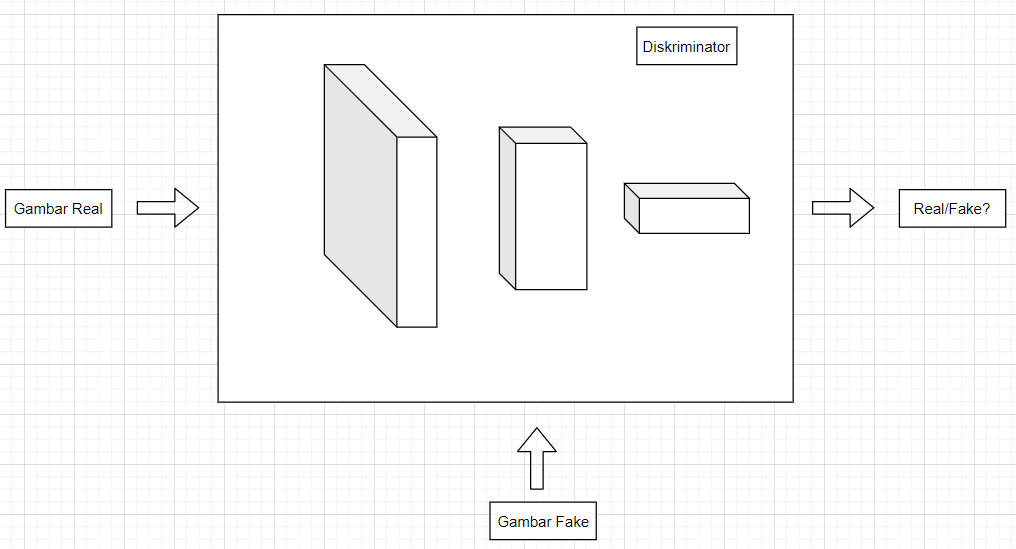
\includegraphics[width=8cm]{figures/1174084/8/teori10.png}
    \centering
    \caption{Teori 10}
\end{figure}		
	

\item Jelaskan bagaimana kaitan output dan input antara generator dan diskriminator tersebut. Jelaskan kenapa inputan dan outputan seperti itu
	\hfill\\
	Pada setiap metode tersebut (Discriminator generator) akan dilakukan pelatihan dan akan dibandingkan hasilnya. Generator akan menghasilkan data baru sesuai dengan hasil latihan dan dari data tersebut, discriminator akan membandingkan dengan data set apakah data tersebut asli atau tidak.
	

\item Jelaskan apa perbedaan antara Kullback-Leibler divergence (KL divergence)/relative entropy, Jensen-Shannon(JS) divergence / information radius(iRaD) / total divergence to the average dalam mengukur kualitas dari model.
	\hfill\\
	relative entropy adalah ukuran dari bagaimana satu distribusi probabilitas berbeda dari yang kedua, distribusi probabilitas referensi, Divergensi Jensen-Shannon adalah ukuran divergensi berprinsip yang selalu terbatas untuk variabel acak terbatas.


\item Jelaskan apa itu fungsi objektif yang berfungsi untuk mengukur kesamaan antara gambar yang dibuat dengan yang asli.
	\hfill\\
	Fungsi objektif adalah fungsi yang digunakan sebagai penujuk berapa nilai kesamaan anatara gambar yang dibuat dengan yang asli
	
\item Jelaskan apa itu scoring algoritma selain mean square error atau cross entropy seperti The Inception Score dan The Frechet Inception distance.
	\hfill\\
	Inception Score digunakan untuk mengukur seberapa realistis output dari GAN, dimana ada dua parameter, yaitu: gambarnya punya variasi dan setiap gambar jelas terlihat seperti sesuatu. Frechet Inception Distance adalah ukuran kesamaan antara dua dataset gambar. Itu terbukti berkorelasi baik dengan penilaian manusia terhadap kualitas visual dan paling sering digunakan untuk mengevaluasi kualitas sampel Generative Adversarial Networks. FID dihitung dengan menghitung jarak Frechet antara dua Gaussians dipasang ke representasi fitur dari jaringan Inception.
	
\item  Jelaskan kelebihan dan kekurangan GAN
	\hfill\\
	Keungungan
GAN Menghasilkan data baru yang bisa hampir mirip dengan data asli. Karena hasil pelatihannya, GAN dapat menghasilkan data gambar, teks, audio, dan video yang dapat dibilang hampir mirip dengan yang aslinya. Berkat hal tersebut, GAN dapat digunakan dalam sistem marketing, e-commerce, games,iklan, dan industri lainnya
GAN mempelajari representasi data secara internal sehingga beberapa masalah pada machine learning dapat diatasi dengan mudah
Discriminator yang sudah dilatih dapat menjadi sebuah classifier atau pendeteksi jika data sudah sesuai. Karena Discriminator yang akan menjadi tidak efisien berkat seringnya dilatih
GAN dapat dilatih menggunakan data yang belum dilabeled

Kerugian
Data saat diproses oleh metode gan tidak konvergensi
Jenis sampel yang dihasilkan oleh generator terbatas karena modenya terbatas
Ketidak seimbangnya antara generator dan discriminator dapat menyebabkan overfitting atau terlalu dekat dengan hasil sampel
Sangat sensitif dengan data yang sudah diinisiasi sebelumnya.
	
\end{enumerate}




\subsection{Praktek}
\begin{enumerate}

\item Jelaskan apa itu 3D convolutions
	\hfill\\
	Konvolusi 3D menerapkan filter 3 dimensi ke dataset dan filter bergerak 3 arah (x, y, z) untuk menghitung representasi fitur level rendah. Bentuk output mereka adalah ruang volume 3 dimensi seperti kubus atau kuboid.

\item Jelaskan dengan kode program arsitektur dari generator networknya, beserta penjelasan input dan output dari generator network.
\lstinputlisting[firstline=31, lastline=63]{src/1174084/8/run.py}

generator ialah g\_loss, Bentuk jaringan Generator dapat dilihat berkebalikan dengan struktur jaringan saraf pada umumnya. Jaringan Generator menerima input sebuah vektor angka z, kemudian mengubahnya menjadi output gambar tiga dimensi.

\item Jelaskan dengan kode program arsitektur dari diskriminator network, beserta penjelasan input dan outputnya.
\lstinputlisting[firstline=65, lastline=105]{src/1174084/8/run.py}

Diskrimanator adalah d\_loss, Jaringan Discriminator merupakan jaringan klasifikasi biner yang menerima input gambar tiga dimensi dan mengeluarkan klasifikasi menyatakan input gambar adalah gambar asli dari dataset atau merupakan gambar buatan Generator. Diskriminator dilatih dengan dataset yang diambil dari Generator, lalu di training untuk membedakan keduanya. Gambar dari Generator yang berhasil di deteksi oleh Diskriminator sebagai gambar fake, akan dikembalikan dengan feedback pke generator. Kini Generator bertugas untuk bisa membuat sekumpulan gambar palsu, yang nantinya dapat dilihat oleh Diskriminator, lalu, Diskriminator tidak bisa membedakan fake dan real.

\item Jelaskan proses training 3D-GANs
	\hfill\\
	proses training 3D gan yaitu dengan melakukan epoch sebanyak yang ditentukan.

\item Jelaskan bagaimana melakukan settingan awal chapter 02 untuk memenuhi semua kebutuhan sebelum melanjutkan ke tahapan persiapan data.
	\hfill\\
	\begin{itemize}
		\item Clone github
		\item Download dataset
		\item Buat folder baru logs dan results
	\end{itemize}

\item Jelaskan tentang dataset yang digunakan, dari mulai tempat unduh, cara membuka dan melihat data. Sampai deskripsi dari isi dataset dengan detail penjelasan setiap folder/file yang membuat orang awam paham.
	\hfill\\
	Dataset yang digunakan yaitu 3DShapeNets yang berisi model model bentuk benda dll, folder train berisi train dan folder test berisi data testing. dan semua data tersebut di simpan didalam folder volumetric\_data.

\item Jelaskan apa itu voxel dengan ilustrasi dan bahasa paling awam.
	\hfill\\
	Volume pixel atau voxel adalah titik dalam ruang tiga dimensi. Sebuah voxel mendefinisikan posisi dengan tiga koordinat dalam arah x, y, dan z. Sebuah voxel adalah unit dasar untuk mewakili gambar 3D.

\item Visualisasikan dataset tersebut dalam tampilan visual plot, jelaskan cara melakukan visualisasinya.
	\hfill\\
	\lstinputlisting[firstline=7, lastline=24]{src/1174084/8/praktek.py}
	langkah-langkah seperti ini :
	import library, load data file .mat dan lakukan read memakai matplotlib
\begin{figure}[H]
    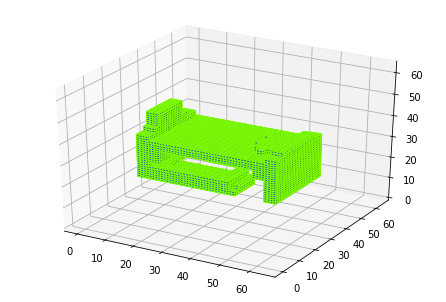
\includegraphics[width=8cm]{figures/1174084/8/bed.png}
    \centering
    \caption{visualisasi}
\end{figure}		
	

\item buka file run.py jelaskan perbaris kode pada fungsi untuk membuat generator yaitu build generator.
	\hfill\\
	\lstinputlisting[firstline=31, lastline=63]{src/1174084/8/run.py}	
	Berfungsi untuk membuat generator yaitu dengan ketentukan gen sebagai variabel dan membuat fungsi atau variabel genmodel lalu dilakukan return.

\item jelaskan juga fungsi untuk membangun diskriminator pada fungsi build discriminator.
	\hfill\\
	\lstinputlisting[firstline=65, lastline=105]{src/1174084/8/run.py}	
	Berfungsi untuk membangun diskriminator berfungsi untuk mendefenisikan seluruh gambar yang sudah di load generator sebagai gambar fake dan real.

\item Jelaskan kode program name = main
	\hfill\\
	Jika interpreter python menjalankan if name main  sebagai program utama, itu ialah menetapkan variabel name  untuk memiliki nilai main. Jika file ini sedang diimpor dari modul lain, name akan ditetapkan ke nama modul. Nama modul tersedia sebagai nilai untuk name variabel global.
\lstinputlisting[firstline=157, lastline=162]{src/1174084/8/run.py}		


\item Jelaskan kode program
\lstinputlisting[firstline=164, lastline=175]{src/1174084/8/run.py}	
	Berfungsi untuk melakukan load dataset dengan ketentuan data yang hanya dalam folder chair pada data train.

\item Jelaskan kode program pembuatan dan kompilasi arsitektur
\lstinputlisting[firstline=177, lastline=189]{src/1174084/8/run.py}	
	Menggunakan Adam sebagai algoritma pengoptimalan dan binary\_crossentropy sebagai kerugian loss.


\item Jelaskan kode program membuat dan melakukan kompilasi model adversarial
\lstinputlisting[firstline=191, lastline=199]{src/1174084/8/run.py}	
	Ini artinya ialah kita memasukkan random vector kedalam generator model lalu membagi 2 yaitu generated example dan real example, dan meneruskan ke diskriminator model sebagai real atau fake

\item Jelaskan kode program Ekstrak dan load data kursi dengan menggunakan fungsi getVoxelsFormat dan get3DImages 
\lstinputlisting[firstline=201, lastline=206]{src/1174084/8/run.py}	
	Berfungsi untuk melakukan load data pada dataset.
	
\item Jelaskan kode program instansiasi TensorBoard yang menambahkan generator dan diskriminator
\lstinputlisting[firstline=208, lastline=212]{src/1174084/8/run.py}	
	Berfungsi untuk membuat tensorboard yang nantinya bisa diakses melalui localhost.

\item Jelaskan kode program, fungsi dari np reshape ones zeros 
\lstinputlisting[firstline=214, lastline=217]{src/1174084/8/run.py}	
	Berfungsi untuk melakukan reshape agar shape yang dihasilkan tidak terlalu besar. Dengan membuat variabel real dan fake.

\item Jelaskan kode, kenapa harus ada perulangan dalam meraih epoch
\lstinputlisting[firstline=219, lastline=226]{src/1174084/8/run.py}	
	Berfungsi untuk melakukan training epoch, karena jika epoch semakin banyak maka kualiatas training yang dihasilkan akan semakin baik.

\item Jelaskan kode program batches
\lstinputlisting[firstline=228, lastline=233]{src/1174084/8/run.py}	
	Batch adalah jumlah file yang akan di training.

\item Jelaskan kode program pengambilan gambar dan noise
\lstinputlisting[firstline=235, lastline=238]{src/1174084/8/run.py}	
	Berfungsi untuk untuk membuat gambar bersih dari noise dan juga menyesuaikan shape.

\item Jelaskan kode program generator gambar palsu
\lstinputlisting[firstline=240, lastline=247]{src/1174084/8/run.py}	
	Berfungsi untuk membuat sample gambar palsu yang akan diteruskan ke diskriminator.
	
\item Jelaskan kode program training diskriminator dengan gambar palsu dari generator dan gambar asli
\lstinputlisting[firstline=249, lastline=260]{src/1174084/8/run.py}	
	Berfungsi untuk membuat diskriminator bisa load gambar fake dan real dari generator, oleh karena itu ada generator loss dan diskriminator loss untuk melihat seberapa baik kualitas yang dihasilkan.

\item Jelaskan kode program training model adversarial yang terdapat generator dan diskriminator
\lstinputlisting[firstline=262, lastline=273]{src/1174084/8/run.py}
	Befungsi untuk melakukan print gloss untuk generator dan juga dloss untuk diskriminator.

\item Jelaskan kode program  generate dan menyimpan gambar 3D setelah beberapa saat setiap epoch
\lstinputlisting[firstline=275, lastline=285]{src/1174084/8/run.py}	
	Mengapa ada perulangan, karena untuk melakukan perbandingan dari hasil yang sudah didapat.

\item Jelaskan kode program  menyimpan average losses setiap epoch
\lstinputlisting[firstline=287, lastline=295]{src/1174084/8/run.py}	
	TensorBoard adalah sebuah aplikasi web localhost untuk memeriksa dan menyelesaikan grafik dari hasil TensorFlow.

\item Jelaskan kode program menyimpan model
\lstinputlisting[firstline=297, lastline=300]{src/1174084/8/run.py}	
	File H5 adalah file data yang disimpan dalam Format Data Hirarki (HDF). Ini berisi array multidimensi data ilmiah.

\item Jelaskan kode program testing model
\lstinputlisting[firstline=302, lastline=321]{src/1174084/8/run.py}	
	Ini adalah tahap akhir untuk melakukan testing dari model yang telah dibuat dan buat model dari yang sudah di create sebelumnya yaitu generator dan diskriminator.

\end{enumerate}


\subsection{Bukti Tidak Plagiat}
\begin{figure}[H]
	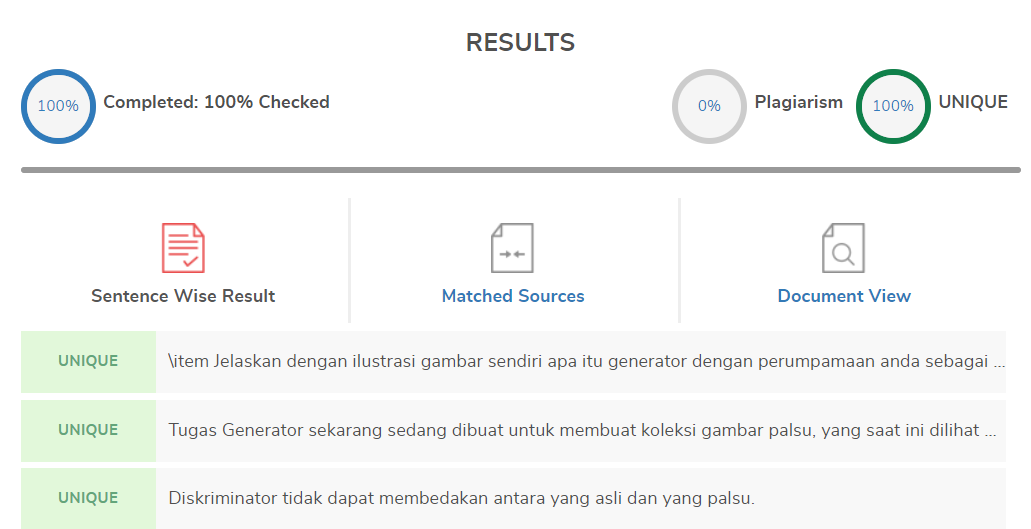
\includegraphics[width=4cm]{figures/1174084/8/plagiarism.png}
	\centering
	\caption{plagiarism}
\end{figure}


\subsection{Link Video Youtube}
https://youtu.be/qETedUr2Le4
